\documentclass[11pt,a4paper]{article}
\usepackage{listings}
\usepackage{graphicx}
\usepackage{color}
\usepackage{textcomp}

\lstset { %
    basicstyle=\footnotesize,
    breaklines=true,
    frame=single,
    numbers=left,
    numbersep=5pt,
    numberstyle=\tiny,
    stepnumber=1,
}

\begin{document}
\title{Soft050 Synth Report}
\date{12/05/2017}
\author{10564011}
\maketitle

\pagebreak

\tableofcontents

\pagebreak

\section{Background}
The program is an audio synthesiser which will be designed to run on Linux operating systems. There is a lack of good audio software availible for Linux, however there is a definite demand for it. The program will provide a configurable musical instrument for the user.

\section{Method}
Haskell with the stack eco-system has been used as the programming language and environment. Functional Reactive Programming techniques with the Reactive Banana libraries have been leveraged in order to provide GUI and MIDI event handling as well as managing the state of the instrument. Reactive Banana was chosen over Wires as it does not require being the "Main Loop" of the program, instead reacting to calls from other functions. \\ \\
The GUI has been built with Glade, which is a graphical GUI design frontend for GTK. Glade produces an XML file which the program reads to create the GUI and define events and behaviors relating to GUI elements. \\ \\
The midi-simple library was used to convert raw MIDI messages from JACK into a more sensible data structure for use within the program, this aids with pattern matching MIDI events.

\section{Analysis}
This program provides a musical instrument with configurable sound qualities which interfaces with JACK for MIDI input and audio output. It aims to provide a low latency response to MIDI input and a simple to use GUI. 

\section{Design}
\subsection{User Interface}
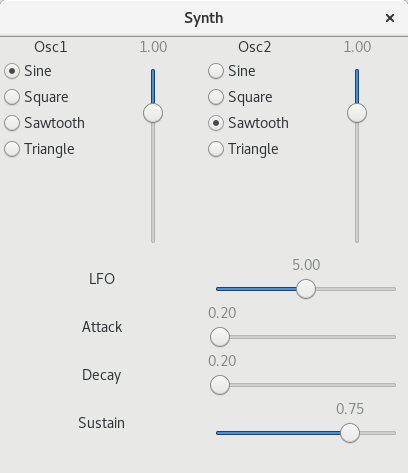
\includegraphics{GUI.png}

\subsection{Code Structure}
The program is split into 5 modules; the Main module which contains the main function (Called on program execution); the JACK module, which has the necessary interface to communicate with JACK; the MIDI module, which provides the helper functions for MIDI event processing; the GUI module, which sets up the event network for the GUI; the Wave module, which defines the functions needed to create the waveforms fed into JACK's output and the Event module in which the main logic behind the event network is defined.

\section{Implementation}
\subsection{foldWaves}
The foldWaves function is an integral part of the program, as it takes the IntMap containing all the Frequencies, Times and Velocities of the current notes being held down, and folds them with the makeWave function to produce a single soundwave which is presented to JACK.

\lstinputlisting[language=Haskell, firstline=49, lastline=53]{../src/Synth/Wave.hs}

The function takes the IntMap and a partially applied makeWave function already containing the GUI settings as parameters. \\
The first part of the function is a lambda being parsed as the first argument to the foldr function. The lambda takes a single note from the IntMap and applies it to the wave function, then it is added to the other notes applied via a pointwise addition from the Linear.Vector library. \\
This fold is embedded inside another lambda function which takes the wave function as an argument. It is fmapped with the wave function since it is in the Behavior functor, and the folding function is not. \\ 
Lastly the fold is applied to the IntMap containing the notes with \textlangle{}*\textrangle{} from Control.Applicative resulting in a single wave function.

\subsection{notesB}
notesB is a Behavior created from the accumulation of MIDI events. It combines the midiNotesE event, which filters just midi note events from midiE, and the runNotes function which either inserts or deletes notes from the IntMap depending on whether a key is pressed of released.

\pagebreak

notesB:
\lstinputlisting[language=Haskell, firstline=42, lastline=42]{../src/Synth/Event.hs} 
isNote:
\lstinputlisting[language=Haskell, firstline=9, lastline=12]{../src/Synth/MIDI.hs} runNotes:
\lstinputlisting[language=Haskell, firstline=23, lastline=34]{../src/Synth/MIDI.hs}

The isNote function takes a MidiMessage from Sound.MIDI and returns True if it is either a NoteOn or NoteOff. \\
The runNotes function takes a MidiMessage filtered by isNote, the velocity of the note and a tick value of the time the MIDI Event occurred and an IntMap in the state before the function was run. \\
It checks to see if the MidiMessage is either NoteOn or NoteOff, then either inserts the relevant data into the IntMap, or deletes a record pertaining to that note.
notesB takes a Behavior accumulated by accumB from Reactive.Banana. accumB takes the empty IntMap as a starting value and the Event created by applied fmap to a lambda function containing runNotes and midiNotesE containing the MidiMessage, velocity and time.

\section{Conclusion}
\subsection{Progess}
6 main features were planned, out of those The Soundwave Generator, Jack Interface, Soundwave Effects and Graphical User Interface were implemented, whereas the Sqlite Database and MIDI file playing ability were omitted. \\

The Sqlite Database was omitted due to time restrictions. The developer didn't feel that the time spent implementing the Sqlite Database would be as valuable as time spent developing other main features of the program. \\

The Midi file playing ability was omitted as the developer felt that this feature went outside of the scope of the program, since the program will accept any MIDI input from JACK, not just that from a keyboard.

\subsection{Review}
Over the course of this project several new technologies have been learnt such as Functional Reactive Programming and GTK. The developer has also greatly expanded their knowledge about applicative functors in Haskell. \\ 
If more time was available the developer would implement features such as a sustain envelope, preset database and a reverb effect. The developer would also implement the ability for mapping GUI Controls to MIDI Controls.
The project has been a success.

\pagebreak

\section{Appendix A: Functional Specification}
\begin{tabular}{ | l | l | l | p{5cm} | }
    \hline
    Functionality & Included & Priority & Notes \\ \hline
    Sine Wave Function & Yes & Must Have & \\ \hline
    Square Wave Function & Yes & Should Have & \\ \hline
    Sawtooth Wave Function & Yes & Should Have & \\ \hline
    Triangle Wave Function & Yes & Should Have & \\ \hline
    MIDI Input & Yes & Should Have & Implemented using JACK \\ \hline
    Audio Output & Yes & Must Have & Implemented using JACK \\ \hline
    Low Latency MIDI Response & Yes & Should Have & \\ \hline
    Low Frequency Oscillator & Yes & Should Have & \\ \hline
    Attack Decay Sustain Envelope & Yes & Could Have & \\ \hline
    Sustain Envelope & No & Could Have & Ommited due to time restraints \\ \hline
    Graphical User Interface & Yes & Must Have & Implemented using GTK \\ \hline
    Radio Button Oscillator Selectors & Yes & Should Have & \\ \hline
    Oscillator Amplitude Scale & Yes & Should Have & \\ \hline
    LFO Frequency Scale & Yes & Should Have & \\ \hline
    ADR Selector Scale & Yes & Could Have & \\ \hline
    Sustain Time Scale & No & Could Have & Sustain not implemented \\ \hline
    Preset Database & No & Should Have & Omitted due to time restraints \\
    \hline
\end{tabular}

\section{Appendix B: Test Plan}
\begin{tabular}{ | p{5cm} | p{5cm} | l | }
    \hline
    Test & Result & Pass/Fail \\ \hline
    Press key on midi input & Sound output & Pass \\ \hline
    Vary velocity of key press & Sound amplitude changes & Pass \\ \hline
    Change note being pressed & Frequency of sound changes & Pass \\ \hline
    Press multiple notes at once & Multiple frequencies of sound & Pass \\ \hline
    Change oscillators & Timbre of sound changes & Pass \\ \hline
    Change oscillator amplitude & Volume of sonud rises & Pass \\ \hline
    Change LFO frequency & Timbre of sound changed & Pass \\ \hline
    Change attack & Note takes longer/shorter to reach full volume & Pass \\ \hline
    Change decay & Note takes loner/shorter to reach sustain volume & Pass \\ \hline
    Change sustain & Sustain volume is quieter / louder & Pass \\ \hline
    Close GUI & GUI closes but program does not & Partial Pass \\
    \hline
\end{tabular}

\section{Appendix C: Full Code}
Main.hs
\lstinputlisting[language=Haskell]{../src/Main.hs}
Synth/JACK.hs
\lstinputlisting[language=Haskell]{../src/Synth/JACK.hs}
Synth/MIDI.hs
\lstinputlisting[language=Haskell]{../src/Synth/MIDI.hs}
Synth/Wave.hs
\lstinputlisting[language=Haskell]{../src/Synth/Wave.hs}
Synth/GUI.hs
\lstinputlisting[language=Haskell]{../src/Synth/GUI.hs}
Synth/Event.hs
\lstinputlisting[language=Haskell]{../src/Synth/Event.hs}
\end{document}
